% ==============================================================================
% CỤM 1 - ĐỀ THAM KHẢO 3 (NĂM HỌC 2026 - 2027)
% ==============================================================================

\begin{bt}%[9D6H18-2]
% nguon: Đề tham khảo Tuyển sinh 10 TP.HCM 2026-2027 – Cụm 1 (Đề 3), Bài 1, trang 7
Cho hàm số $(P): y = x^2$.
\begin{enumerate}[a)]
	\item Vẽ đồ thị $(P)$.
	\item Tìm tọa độ các điểm $M$ thuộc $(P)$ có tung độ bằng $25$.
\end{enumerate}
\loigiai{
	\begin{enumerate}[a)]
		\item Bảng giá trị tương ứng giữa $x$ và $y$:
		\begin{center}
		\begin{tabular}{|c|c|c|c|c|c|}
		\hline
		$x$ & $-2$ & $-1$ & $0$ & $1$ & $2$ \\
		\hline
		$y = x^2$ & $4$ & $1$ & $0$ & $1$ & $4$ \\
		\hline
		\end{tabular}
		\end{center}
		Đồ thị $(P)$ là đường cong parabol đi qua gốc tọa độ $O(0; 0)$ và các điểm $(-2; 4)$, $(-1; 1)$, $(1; 1)$, $(2; 4)$, nhận trục tung $Oy$ làm trục đối xứng và có bề lõm quay lên trên.
		\begin{center}
		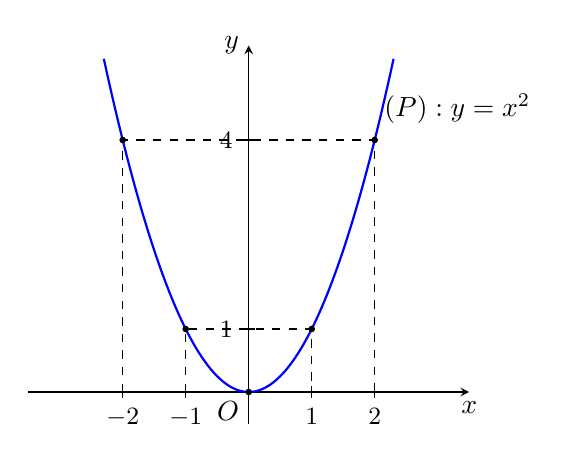
\begin{tikzpicture}[>=stealth, scale=0.8]
			\draw[->] (-3.5,0) -- (3.5,0) node[below] {$x$};
			\draw[->] (0,-0.5) -- (0,5.5) node[left] {$y$};
			\draw (0,0) node[below left] {$O$};
			\foreach \x in {-2,-1,1,2}
				\draw (\x,0.1) -- (\x,-0.1) node[below] {\small $\x$};
			\foreach \y in {1,4}
				\draw (0.1,\y) -- (-0.1,\y) node[left] {\small $\y$};
			\draw[dashed] (-2,0) -- (-2,4) -- (2,4) -- (2,0);
			\draw[dashed] (-1,0) -- (-1,1) -- (1,1) -- (1,0);
			\draw[smooth,samples=100,domain=-2.3:2.3,thick,blue] plot(\x,{(\x)^2});
			\node[right] at (2,4.5) {$(P): y=x^2$};
			\fill (-2,4) circle (1.5pt) (-1,1) circle (1.5pt) (0,0) circle (1.5pt) (1,1) circle (1.5pt) (2,4) circle (1.5pt);
		\end{tikzpicture}
		\end{center}
		\item Điểm $M(x; y) \in (P)$ có tung độ bằng $25$ nên $y = 25$.\\
		Thay $y = 25$ vào phương trình parabol $(P)$, ta có:
		$$x^2 = 25 \iff x^2 - 25 = 0 \iff x = 5 \text{ hoặc } x = -5.$$
		Với $x = 5 \implies y = 25$, ta được điểm $M_1(5; 25)$.\\
		Với $x = -5 \implies y = 25$, ta được điểm $M_2(-5; 25)$.\\
		Vậy có hai điểm thỏa mãn yêu cầu bài toán là $(5; 25)$ và $(-5; 25)$.
	\end{enumerate}
}
\end{bt}

\begin{bt}%[9D6H20-2]
% nguon: Đề tham khảo Tuyển sinh 10 TP.HCM 2026-2027 – Cụm 1 (Đề 3), Bài 2, trang 7
Cho phương trình: $2x^2 - 4x + 1 = 0$.
\begin{enumerate}[a)]
	\item Chứng minh phương trình trên luôn có hai nghiệm phân biệt $x_1, x_2$.
	\item Không giải phương trình, hãy tính giá trị của biểu thức:
	$$A = x_1(x_1 + 2026) + x_2(x_2 + 2027) - x_2$$
\end{enumerate}
\loigiai{
	\begin{enumerate}[a)]
		\item Xét phương trình $2x^2 - 4x + 1 = 0$ có các hệ số $a = 2, b = -4, c = 1$.\\
		Ta có:
		$$\Delta' = (b')^2 - ac = (-2)^2 - 2 \cdot 1 = 4 - 2 = 2 > 0.$$
		Vì $\Delta' > 0$ nên phương trình luôn có hai nghiệm phân biệt $x_1, x_2$.
		\item Theo định lý Vi-ét, ta có:
		$$\begin{cases} x_1 + x_2 = -\dfrac{b}{a} = -\dfrac{-4}{2} = 2 \\ x_1 x_2 = \dfrac{c}{a} = \dfrac{1}{2} \end{cases}$$
		Từ đó tính được:
		$$x_1^2 + x_2^2 = (x_1 + x_2)^2 - 2x_1 x_2 = 2^2 - 2 \cdot \frac{1}{2} = 4 - 1 = 3.$$
		Khai triển và rút gọn biểu thức $A$:
		\begin{align*}
		A &= x_1(x_1 + 2026) + x_2(x_2 + 2027) - x_2 \\
		  &= x_1^2 + 2026x_1 + x_2^2 + 2027x_2 - x_2 \\
		  &= (x_1^2 + x_2^2) + 2026x_1 + 2026x_2 \\
		  &= (x_1^2 + x_2^2) + 2026(x_1 + x_2)
		\end{align*}
		Thay các giá trị $x_1^2 + x_2^2 = 3$ và $x_1 + x_2 = 2$ vào biểu thức $A$, ta được:
		$$A = 3 + 2026 \cdot 2 = 3 + 4052 = 4055.$$
		Vậy $A = 4055$.
	\end{enumerate}
}
\end{bt}

\begin{bt}%[9D8H26-3]
% nguon: Đề tham khảo Tuyển sinh 10 TP.HCM 2026-2027 – Cụm 1 (Đề 3), Bài 3, trang 7
Kết quả xếp loại học tập học kì I của học sinh một trường THCS được ghi nhận như sau:
\begin{itemize}
	\item Khối 6: $221$ học sinh Tốt, $305$ học sinh Khá, $50$ học sinh Đạt.
	\item Khối 7: $215$ học sinh Tốt, $292$ học sinh Khá, $61$ học sinh Đạt.
	\item Khối 8: $207$ học sinh Tốt, $275$ học sinh Khá, $77$ học sinh Đạt.
	\item Khối 9: $193$ học sinh Tốt, $318$ học sinh Khá, $75$ học sinh Đạt.
\end{itemize}
\begin{enumerate}[a)]
	\item Toàn trường có bao nhiêu học sinh đạt kết quả học tập Tốt ở học kì I?
	\item Chọn ngẫu nhiên một học sinh của trường, tính xác suất của các biến cố sau:
	\begin{itemize}
		\item Biến cố $A$: "Học sinh được chọn có kết quả học tập Tốt".
		\item Biến cố $B$: "Học sinh được chọn có kết quả học tập từ Khá trở lên".
	\end{itemize}
\end{enumerate}
\loigiai{
	\begin{enumerate}[a)]
		\item Số học sinh đạt kết quả học tập Tốt ở học kì I của toàn trường là:
		$$221 + 215 + 207 + 193 = 836\text{ (học sinh)}.$$
		\item Tổng số học sinh của toàn trường là:
		\begin{align*}
		n(\Omega) &= (221 + 305 + 50) + (215 + 292 + 61) + (207 + 275 + 77) + (193 + 318 + 75) \\
		          &= 576 + 568 + 559 + 601 = 2304\text{ (học sinh)}.
		\end{align*}
		\begin{itemize}
			\item Biến cố $A$: "Học sinh được chọn có kết quả học tập Tốt".\\
			Số kết quả thuận lợi cho biến cố $A$ là $n(A) = 836$.\\
			Xác suất của biến cố $A$ là:
			$$P(A) = \frac{n(A)}{n(\Omega)} = \frac{836}{2304} = \frac{209}{576}.$$
			\item Biến cố $B$: "Học sinh được chọn có kết quả học tập từ Khá trở lên".\\
			Số học sinh đạt kết quả Khá của toàn trường là:
			$$305 + 292 + 275 + 318 = 1190\text{ (học sinh)}.$$
			Số kết quả thuận lợi cho biến cố $B$ (gồm học sinh Tốt và Khá) là:
			$$n(B) = 836 + 1190 = 2026\text{ (học sinh)}.$$
			Xác suất của biến cố $B$ là:
			$$P(B) = \frac{n(B)}{n(\Omega)} = \frac{2026}{2304} = \frac{1013}{1152}.$$
		\end{itemize}
	\end{enumerate}
}
\end{bt}

\begin{bt}%[9D6V21-3]
% nguon: Đề tham khảo Tuyển sinh 10 TP.HCM 2026-2027 – Cụm 1 (Đề 3), Bài 4, trang 7
Anh Tâm có một mảnh vườn hình vuông với diện tích bằng $81\text{ m}^2$. Anh muốn mở rộng mảnh vườn này thành mảnh vườn hình chữ nhật sao cho các cạnh của hình chữ nhật cách các cạnh của hình vuông tương ứng các khoảng cách là $x$, $2x$, $3x$ (cạnh dưới và cạnh phải cách $x$, cạnh trên cách $2x$, cạnh trái cách $3x$, với $x > 0$, tính theo mét).
\begin{enumerate}[a)]
	\item Viết biểu thức $S$ biểu thị diện tích của mảnh vườn sau khi mở rộng theo $x$.
	\item Biết rằng sau khi mở rộng, diện tích của mảnh vườn tăng thêm $810\text{ m}^2$. Tìm giá trị của $x$.
\end{enumerate}
\loigiai{
	\begin{enumerate}[a)]
		\item Vì mảnh vườn ban đầu là hình vuông có diện tích $81\text{ m}^2$ nên độ dài cạnh hình vuông là:
		$$\sqrt{81} = 9\text{ (m)}.$$
		Sau khi mở rộng thành hình chữ nhật:
		\begin{itemize}
			\item Chiều dài mới gồm cạnh hình vuông cộng thêm khoảng cách mở rộng về hai phía trái và phải:
			$$9 + 3x + x = 9 + 4x\text{ (m)}.$$
			\item Chiều rộng mới gồm cạnh hình vuông cộng thêm khoảng cách mở rộng về hai phía trên và dưới:
			$$9 + 2x + x = 9 + 3x\text{ (m)}.$$
		\end{itemize}
		Diện tích $S$ của mảnh vườn hình chữ nhật sau khi mở rộng là:
		$$S = (9 + 4x)(9 + 3x) = 81 + 27x + 36x + 12x^2 = 12x^2 + 63x + 81\text{ (m}^2\text{)}.$$
		\item Theo đề bài, sau khi mở rộng diện tích mảnh vườn tăng thêm $810\text{ m}^2$, nên diện tích mới là:
		$$S = 81 + 810 = 891\text{ (m}^2\text{)}.$$
		Ta có phương trình:
		$$12x^2 + 63x + 81 = 891 \iff 12x^2 + 63x - 810 = 0 \iff 4x^2 + 21x - 270 = 0.$$
		Phương trình có $\Delta = 21^2 - 4 \cdot 4 \cdot (-270) = 441 + 4320 = 4761 = 69^2 > 0$.\\
		Suy ra phương trình có hai nghiệm:
		$$x_1 = \frac{-21 + 69}{8} = 6\text{ (nhận do } x > 0), \quad x_2 = \frac{-21 - 69}{8} = -\frac{45}{4}\text{ (loại)}.$$
		Vậy giá trị của $x$ là $6\text{ m}$.
	\end{enumerate}
}
\end{bt}

\begin{bt}%[9H0V31-3]
% nguon: Đề tham khảo Tuyển sinh 10 TP.HCM 2026-2027 – Cụm 1 (Đề 3), Bài 5, trang 8
Một viên gạch ống hình hộp chữ nhật có kích thước dài $20\text{ cm}$, rộng $8\text{ cm}$ và cao $8\text{ cm}$. Bên trong viên gạch có bốn lỗ rỗng hình trụ bằng nhau chạy suốt chiều dài viên gạch, mỗi lỗ có đường kính đáy là $2{,}5\text{ cm}$.
\begin{enumerate}[a)]
	\item Tính thể tích đất sét cần dùng để làm một viên gạch (lấy $\pi = 3{,}14$).
	\item Bác Tư xây nhà cần dùng $10$ thiên gạch ($1$ thiên $= 1\,000$ viên), giá mỗi viên gạch là $2\,500$ đồng. Bác Tư đã mua dư $2\%$ số lượng gạch cần dùng dự phòng hư hao khi thi công. Tính tổng số tiền Bác Tư phải trả để mua gạch.
\end{enumerate}
\loigiai{
	\begin{enumerate}[a)]
		\item Thể tích toàn phần của khối hình hộp chữ nhật bao ngoài viên gạch là:
		$$V_{\text{hộp}} = 20 \cdot 8 \cdot 8 = 1280\text{ (cm}^3\text{)}.$$
		Bán kính đáy của mỗi lỗ rỗng hình trụ là:
		$$r = \frac{2{,}5}{2} = 1{,}25\text{ (cm)}.$$
		Tổng thể tích của cả $4$ lỗ rỗng hình trụ là:
		$$V_{\text{lỗ}} = 4 \cdot (\pi r^2 h) = 4 \cdot \pi \cdot 1{,}25^2 \cdot 20 = 125\pi = 125 \cdot 3{,}14 = 392{,}5\text{ (cm}^3\text{)}.$$
		Thể tích đất sét thực tế cần dùng để sản xuất một viên gạch là:
		$$V = V_{\text{hộp}} - V_{\text{lỗ}} = 1280 - 392{,}5 = 887{,}5\text{ (cm}^3\text{)}.$$
		\item Số lượng gạch cần dùng là $10$ thiên gạch, tương ứng với:
		$$10 \cdot 1\,000 = 10\,000\text{ (viên)}.$$
		Do Bác Tư mua thêm $2\%$ dự phòng hao hụt nên số lượng gạch thực tế Bác Tư mua là:
		$$10\,000 + 10\,000 \cdot 2\% = 10\,200\text{ (viên)}.$$
		Tổng số tiền Bác Tư phải trả là:
		$$10\,200 \cdot 2\,500 = 25\,500\,000\text{ (đồng)}.$$
		\textit{(Nếu tính tròn theo đúng $10$ thiên gạch chưa gồm phần dư thì chi phí là $10\,000 \times 2\,500 = 25\,000\,000$ đồng).}
	\end{enumerate}
}
\end{bt}

\begin{bt}%[9D1H3-4]
% nguon: Đề tham khảo Tuyển sinh 10 TP.HCM 2026-2027 – Cụm 1 (Đề 3), Bài 6, trang 8
Trong một trại nuôi tôm sú giống, kỹ sư đang có hai nguồn nước mặn với nồng độ mặn khác nhau. Để đạt được độ mặn mong muốn, kỹ sư đã thử nghiệm hai tỉ lệ pha chế:
\begin{itemize}
	\item Lấy $200\text{ ml}$ nguồn thứ nhất pha với $300\text{ ml}$ nguồn thứ hai thì được dung dịch mới có nồng độ mặn $27\%$.
	\item Lấy $300\text{ ml}$ nguồn thứ nhất pha với $200\text{ ml}$ nguồn thứ hai thì được dung dịch mới có nồng độ mặn $28\%$.
\end{itemize}
\begin{enumerate}[a)]
	\item Tính nồng độ mặn của mỗi nguồn nước mặn ban đầu.
	\item Mỗi hồ nuôi tôm cần $4\text{ m}^3$ nước có nồng độ mặn $28\%$. Hỏi cần lấy bao nhiêu mét khối nước từ mỗi nguồn nước mặn ban đầu?
\end{enumerate}
\loigiai{
	\begin{enumerate}[a)]
		\item Gọi nồng độ mặn của nguồn nước thứ nhất và nguồn nước thứ hai lần lượt là $x$ và $y$ ($\%$) ($x, y > 0$).\\
		Lượng muối nguyên chất trong $200\text{ ml}$ nguồn một là $200 \cdot \dfrac{x}{100} = 2x\text{ (ml)}$.\\
		Lượng muối nguyên chất trong $300\text{ ml}$ nguồn hai là $300 \cdot \dfrac{y}{100} = 3y\text{ (ml)}$.\\
		Vì pha $200\text{ ml}$ nguồn một với $300\text{ ml}$ nguồn hai được $500\text{ ml}$ dung dịch nồng độ $27\%$ nên:
		$$2x + 3y = 500 \cdot \frac{27}{100} \iff 2x + 3y = 135 \quad (1)$$
		Tương tự, pha $300\text{ ml}$ nguồn một với $200\text{ ml}$ nguồn hai được $500\text{ ml}$ dung dịch nồng độ $28\%$ nên:
		$$3x + 2y = 500 \cdot \frac{28}{100} \iff 3x + 2y = 140 \quad (2)$$
		Từ $(1)$ và $(2)$, ta có hệ phương trình:
		$$\begin{cases} 2x + 3y = 135 \\ 3x + 2y = 140 \end{cases} \iff \begin{cases} 6x + 9y = 405 \\ 6x + 4y = 280 \end{cases} \iff \begin{cases} 5y = 125 \\ 2x + 3y = 135 \end{cases} \iff \begin{cases} x = 30 \\ y = 25 \end{cases}\text{ (thỏa mãn).}$$
		Vậy nồng độ mặn của nguồn thứ nhất là $30\%$ và nguồn thứ hai là $25\%$.
		\item Gọi thể tích nước cần lấy từ nguồn một ($30\%$) và nguồn hai ($25\%$) lần lượt là $u$ và $v$ ($\text{m}^3$) ($u, v > 0$).\\
		Tổng thể tích nước cần cho hồ là $4\text{ m}^3$, ta có phương trình:
		$$u + v = 4 \quad (3)$$
		Lượng muối có trong $4\text{ m}^3$ nước nồng độ $28\%$ là:
		$$0{,}3u + 0{,}25v = 4 \cdot 28\% = 1{,}12 \quad (4)$$
		Từ $(3)$ và $(4)$, ta có hệ phương trình:
		$$\begin{cases} u + v = 4 \\ 0{,}3u + 0{,}25v = 1{,}12 \end{cases} \iff \begin{cases} 0{,}25u + 0{,}25v = 1 \\ 0{,}3u + 0{,}25v = 1{,}12 \end{cases} \iff \begin{cases} 0{,}05u = 0{,}12 \\ u + v = 4 \end{cases} \iff \begin{cases} u = 2{,}4 \\ v = 1{,}6 \end{cases}\text{ (thỏa mãn).}$$
		Vậy cần lấy $2{,}4\text{ m}^3$ nước từ nguồn thứ nhất và $1{,}6\text{ m}^3$ nước từ nguồn thứ hai.
	\end{enumerate}
}
\end{bt}

\begin{bt}%[9H9C29-3]
% nguon: Đề tham khảo Tuyển sinh 10 TP.HCM 2026-2027 – Cụm 1 (Đề 3), Bài 7, trang 8
Cho tam giác $ABC$ có ba góc nhọn ($AB < AC$) nội tiếp đường tròn $(O; R)$. Hai đường cao $AD, BE$ của tam giác $ABC$ cắt nhau tại trực tâm $H$. Gọi $M, N$ lần lượt là giao điểm của đường tròn $(O)$ với các tia $BE, AD$ ($M \neq B, N \neq A$).
\begin{enumerate}[a)]
	\item Chứng minh tứ giác $ABDE$ nội tiếp và xác định tâm $I$ của đường tròn này, từ đó suy ra $DE \parallel MN$.
	\item Kẻ đường kính $CK$ của đường tròn $(O)$. Chứng minh tứ giác $AKBH$ là hình bình hành và suy ra ba điểm $H, I, K$ thẳng hàng.
	\item Trong trường hợp $\widehat{BCA} = 60^\circ$, chứng minh $DE = \dfrac{1}{2}AB$ và tính diện tích hình viên phân giới hạn bởi cung nhỏ $DE$ và dây cung $DE$ của đường tròn $(I)$ theo $R$.
\end{enumerate}
\loigiai{
	\begin{center}
	\begin{tikzpicture}[scale=1]
		\coordinate (O) at (0,0);
		\def\R{3}
		\draw[thick] (O) circle (\R);
		\coordinate (A) at (75:\R);
		\coordinate (B) at (200:\R);
		\coordinate (C) at (-20:\R);
		
		\coordinate (D) at ($(B)!(A)!(C)$);
		\coordinate (E) at ($(A)!(B)!(C)$);
		\coordinate (H) at (intersection of A--D and B--E);
		
		\coordinate (K) at ($(O)!-1!(C)$);
		\coordinate (I) at ($(A)!0.5!(B)$);
		
		\coordinate (M) at (105:\R);
		\coordinate (N) at (275:\R);
		
		\draw[thick] (A) -- (B) -- (C) -- cycle;
		\draw[thick, blue] (A) -- (D);
		\draw[thick, blue] (B) -- (E);
		\draw[dashed] (D) -- (N);
		\draw[dashed] (E) -- (M);
		\draw[thick, red] (D) -- (E);
		\draw[dashed] (M) -- (N);
		\draw[thick] (C) -- (K);
		\draw[dashed] (A) -- (K) -- (B);
		\draw[dashed] (H) -- (K);
		
		\fill (A) circle (1.5pt) node[above] {$A$};
		\fill (B) circle (1.5pt) node[below left] {$B$};
		\fill (C) circle (1.5pt) node[below right] {$C$};
		\fill (D) circle (1.5pt) node[below] {$D$};
		\fill (E) circle (1.5pt) node[above right] {$E$};
		\fill (H) circle (1.5pt) node[below left] {$H$};
		\fill (O) circle (1.5pt) node[right] {$O$};
		\fill (K) circle (1.5pt) node[above left] {$K$};
		\fill (I) circle (1.5pt) node[above left] {$I$};
		\fill (M) circle (1.5pt) node[above left] {$M$};
		\fill (N) circle (1.5pt) node[below] {$N$};
	\end{tikzpicture}
	\end{center}
	\begin{enumerate}[a)]
		\item Xét tam giác $AEB$ vuông tại $E$ (do $BE \perp AC$) nên tam giác $AEB$ nội tiếp đường tròn đường kính $AB$.\\
		Xét tam giác $ADB$ vuông tại $D$ (do $AD \perp BC$) nên tam giác $ADB$ nội tiếp đường tròn đường kính $AB$.\\
		Do đó bốn điểm $A, B, D, E$ cùng thuộc đường tròn đường kính $AB$, suy ra tứ giác $ABDE$ nội tiếp đường tròn có tâm $I$ là trung điểm của $AB$.\\
		Trong tứ giác nội tiếp $ABDE$, ta có:
		$$\widehat{BDE} = \widehat{BAE} \quad (\text{hai góc nội tiếp cùng chắn cung } BE).$$
		Trong đường tròn $(O)$, ta có:
		$$\widehat{BMN} = \widehat{BAN} \quad (\text{hai góc nội tiếp cùng chắn cung } BN).$$
		Mà điểm $E$ nằm trên cạnh $AC$ và điểm $N$ nằm trên tia $AD$ nên $\widehat{BAE} = \widehat{BAC} = \widehat{BAN}$.\\
		Suy ra $\widehat{BDE} = \widehat{BMN}$.\\
		Hai góc này ở vị trí đồng vị nên $DE \parallel MN$.
		\item Ta có $\widehat{KAC} = 90^\circ$ (góc nội tiếp chắn nửa đường tròn đường kính $KC$), suy ra $KA \perp AC$.\\
		Mà $BE \perp AC$ (do $BE$ là đường cao) $\implies KA \parallel BH$.\\
		Tương tự, $\widehat{KBC} = 90^\circ$ (góc nội tiếp chắn nửa đường tròn đường kính $KC$), suy ra $KB \perp BC$.\\
		Mà $AD \perp BC$ (do $AD$ là đường cao) $\implies KB \parallel AH$.\\
		Tứ giác $AKBH$ có các cặp cạnh đối song song nên là hình bình hành.\\
		Vì $I$ là trung điểm của đường chéo $AB$ nên $I$ cũng là trung điểm của đường chéo $HK$.\\
		Vậy ba điểm $H, I, K$ thẳng hàng.
		\item Xét $\Delta CDE$ và $\Delta CAB$ có:
		$$\widehat{C}\text{ là góc chung và } \widehat{CDE} = \widehat{CAB}\text{ (cùng bù với } \widehat{BDE}\text{)}.$$
		Suy ra $\Delta CDE \backsim \Delta CAB$ (g-g), do đó:
		$$\frac{DE}{AB} = \frac{CD}{CA} = \cos \widehat{BCA} = \cos 60^\circ = \frac{1}{2} \implies DE = \frac{1}{2}AB.$$
		Kẻ đường kính $AQ$ của đường tròn $(O)$.\\
		Ta có $\widehat{ABQ} = 90^\circ$ và $\widehat{AQB} = \widehat{ACB} = 60^\circ$ (hai góc nội tiếp cùng chắn cung $AB$).\\
		Xét tam giác vuông $ABQ$ vuông tại $B$:
		$$AB = AQ \cdot \sin \widehat{AQB} = 2R \cdot \sin 60^\circ = R\sqrt{3}.$$
		Suy ra bán kính của đường tròn $(I)$ là:
		$$R_I = \frac{AB}{2} = \frac{R\sqrt{3}}{2}.$$
		Tam giác $IDE$ có $ID = IE = R_I$ và $DE = \dfrac{1}{2}AB = R_I$, do đó $\Delta IDE$ là tam giác đều cạnh $R_I = \dfrac{R\sqrt{3}}{2}$, suy ra $\widehat{DIE} = 60^\circ$.\\
		Diện tích hình quạt tròn $IDE$ là:
		$$S_{\text{quạt}} = \frac{\pi R_I^2 \cdot 60^\circ}{360^\circ} = \frac{\pi \cdot \left(\frac{R\sqrt{3}}{2}\right)^2}{6} = \frac{\pi R^2}{8}.$$
		Diện tích tam giác đều $IDE$ là:
		$$S_{\Delta IDE} = \frac{R_I^2 \sqrt{3}}{4} = \frac{\left(\frac{R\sqrt{3}}{2}\right)^2 \sqrt{3}}{4} = \frac{3R^2\sqrt{3}}{16}.$$
		Diện tích hình viên phân giới hạn bởi cung nhỏ $DE$ và dây cung $DE$ là:
		$$S = S_{\text{quạt}} - S_{\Delta IDE} = \frac{\pi R^2}{8} - \frac{3R^2\sqrt{3}}{16} = \frac{(2\pi - 3\sqrt{3})R^2}{16}.$$
	\end{enumerate}
}
\end{bt}

% ==============================================================================
% CỤM 2 - ĐỀ THAM KHẢO 1 (NĂM HỌC 2026 - 2027)
% ==============================================================================

\begin{bt}%[9D6H18-2]
% nguon: Đề tham khảo Tuyển sinh 10 TP.HCM 2026-2027 – Cụm 2 (Đề 1), Bài 1, trang 9
Cho hàm số $(P): y = \dfrac{3}{2}x^2$.
\begin{enumerate}[a)]
	\item Vẽ đồ thị $(P)$ trên hệ trục tọa độ.
	\item Tìm tọa độ các điểm thuộc $(P)$ có tung độ bằng $24$.
\end{enumerate}
\loigiai{
	\begin{enumerate}[a)]
		\item Bảng giá trị tương ứng giữa $x$ và $y$:
		\begin{center}
		\begin{tabular}{|c|c|c|c|c|c|}
		\hline
		$x$ & $-2$ & $-1$ & $0$ & $1$ & $2$ \\
		\hline
		$y = \dfrac{3}{2}x^2$ & $6$ & $1{,}5$ & $0$ & $1{,}5$ & $6$ \\
		\hline
		\end{tabular}
		\end{center}
		Đồ thị $(P)$ là đường cong parabol đi qua gốc tọa độ $O(0; 0)$ và các điểm $(-2; 6)$, $(-1; 1{,}5)$, $(1; 1{,}5)$, $(2; 6)$, có bề lõm quay lên trên và nhận trục tung $Oy$ làm trục đối xứng.
		\begin{center}
		\begin{tikzpicture}[>=stealth, scale=0.8]
			\draw[->] (-3.5,0) -- (3.5,0) node[below] {$x$};
			\draw[->] (0,-0.5) -- (0,7) node[left] {$y$};
			\draw (0,0) node[below left] {$O$};
			\foreach \x in {-2,-1,1,2}
				\draw (\x,0.1) -- (\x,-0.1) node[below] {\small $\x$};
			\foreach \y in {1.5,6}
				\draw (0.1,\y) -- (-0.1,\y) node[left] {\small $\y$};
			\draw[dashed] (-2,0) -- (-2,6) -- (2,6) -- (2,0);
			\draw[dashed] (-1,0) -- (-1,1.5) -- (1,1.5) -- (1,0);
			\draw[smooth,samples=100,domain=-2.1:2.1,thick,blue] plot(\x,{1.5*(\x)^2});
			\node[right] at (1.8,6.5) {$(P): y=\dfrac{3}{2}x^2$};
			\fill (-2,6) circle (1.5pt) (-1,1.5) circle (1.5pt) (0,0) circle (1.5pt) (1,1.5) circle (1.5pt) (2,6) circle (1.5pt);
		\end{tikzpicture}
		\end{center}
		\item Gọi điểm cần tìm là $M(x; y) \in (P)$. Theo đề bài, tung độ của điểm đó bằng $24$, tức $y = 24$.\\
		Thay $y = 24$ vào phương trình parabol $(P)$, ta có:
		$$\frac{3}{2}x^2 = 24 \iff x^2 = 24 \cdot \frac{2}{3} = 16 \iff x = 4 \text{ hoặc } x = -4.$$
		Với $x = 4 \implies y = 24$, ta có điểm $M_1(4; 24)$.\\
		Với $x = -4 \implies y = 24$, ta có điểm $M_2(-4; 24)$.\\
		Vậy có hai điểm thuộc $(P)$ có tung độ bằng $24$ là $(4; 24)$ và $(-4; 24)$.
	\end{enumerate}
}
\end{bt}

\begin{bt}%[9D6H20-2]
% nguon: Đề tham khảo Tuyển sinh 10 TP.HCM 2026-2027 – Cụm 2 (Đề 1), Bài 2, trang 9
Cho phương trình: $-3x^2 + 2x + 4 = 0$.
\begin{enumerate}[a)]
	\item Chứng minh phương trình trên luôn có hai nghiệm phân biệt.
	\item Không giải phương trình, hãy tính giá trị của biểu thức:
	$$A = \frac{2x_1}{x_2} + \frac{2x_2}{x_1}$$
\end{enumerate}
\loigiai{
	\begin{enumerate}[a)]
		\item Xét phương trình $-3x^2 + 2x + 4 = 0$ có các hệ số $a = -3, b' = 1, c = 4$.\\
		Vì $a \cdot c = (-3) \cdot 4 = -12 < 0$ nên phương trình luôn có hai nghiệm phân biệt trái dấu $x_1, x_2$.\\
		\textit{(Cách khác: $\Delta' = 1^2 - (-3) \cdot 4 = 1 + 12 = 13 > 0$ nên phương trình luôn có hai nghiệm phân biệt).}
		\item Theo định lý Vi-ét, ta có:
		$$\begin{cases} x_1 + x_2 = -\dfrac{b}{a} = -\dfrac{2}{-3} = \dfrac{2}{3} \\ x_1 x_2 = \dfrac{c}{a} = -\dfrac{4}{3} \end{cases}$$
		Từ đó tính được:
		$$x_1^2 + x_2^2 = (x_1 + x_2)^2 - 2x_1 x_2 = \left(\frac{2}{3}\right)^2 - 2 \cdot \left(-\frac{4}{3}\right) = \frac{4}{9} + \frac{8}{3} = \frac{28}{9}.$$
		Biến đổi biểu thức $A$:
		$$A = \frac{2x_1}{x_2} + \frac{2x_2}{x_1} = 2 \cdot \left(\frac{x_1^2 + x_2^2}{x_1 x_2}\right).$$
		Thay các giá trị tương ứng vào, ta được:
		$$A = 2 \cdot \frac{\frac{28}{9}}{-\frac{4}{3}} = 2 \cdot \left(\frac{28}{9} \cdot \frac{-3}{4}\right) = 2 \cdot \left(-\frac{7}{3}\right) = -\frac{14}{3}.$$
		Vậy $A = -\dfrac{14}{3}$.
	\end{enumerate}
}
\end{bt}

\begin{bt}%[9D8H26-3]
% nguon: Đề tham khảo Tuyển sinh 10 TP.HCM 2026-2027 – Cụm 2 (Đề 1), Bài 3, trang 9
Trong một siêu thị tiện lợi có ba khách hàng Phúc, Bình, An cùng đến quầy thu ngân tại một thời điểm. Nhân viên thu ngân sẽ chọn lần lượt từng khách hàng để thực hiện thanh toán.
\begin{enumerate}[a)]
	\item Có tất cả bao nhiêu kết quả có thể xảy ra? Liệt kê tất cả các kết quả có thể xảy ra của phép thử trên.
	\item Tính xác suất của mỗi biến cố sau:
	\begin{itemize}
		\item Biến cố $A$: "Phúc được thanh toán cuối cùng".
		\item Biến cố $B$: "An được thanh toán trước Bình".
	\end{itemize}
\end{enumerate}
\loigiai{
	\begin{enumerate}[a)]
		\item Ký hiệu ba khách hàng là Phúc ($P$), Bình ($B$) và An ($A$).\\
		Mỗi thứ tự thanh toán lần lượt cho ba khách hàng là một hoán vị của bộ ba khách hàng $(P, B, A)$.\\
		Tất cả các kết quả có thể xảy ra của phép thử là:
		$$\Omega = \{(P, B, A);\, (P, A, B);\, (B, P, A);\, (B, A, P);\, (A, P, B);\, (A, B, P)\}.$$
		Số kết quả có thể xảy ra là:
		$$n(\Omega) = 3! = 6.$$
		\item Xác suất của các biến cố:
		\begin{itemize}
			\item Biến cố $A$: "Phúc được thanh toán cuối cùng".\\
			Các kết quả thuận lợi cho biến cố $A$ là các thứ tự có $P$ ở vị trí thứ ba:
			$$(B, A, P);\, (A, B, P).$$
			Số kết quả thuận lợi là $n(A) = 2$.\\
			Xác suất của biến cố $A$ là:
			$$P(A) = \frac{n(A)}{n(\Omega)} = \frac{2}{6} = \frac{1}{3}.$$
			\item Biến cố $B$: "An được thanh toán trước Bình".\\
			Các kết quả thuận lợi cho biến cố $B$ là các thứ tự mà $A$ đứng trước $B$:
			$$(A, B, P);\, (A, P, B);\, (P, A, B).$$
			Số kết quả thuận lợi là $n(B) = 3$.\\
			Xác suất của biến cố $B$ là:
			$$P(B) = \frac{n(B)}{n(\Omega)} = \frac{3}{6} = \frac{1}{2} = 0{,}5.$$
		\end{itemize}
	\end{enumerate}
}
\end{bt}

\begin{bt}%[9D6V21-3]
% nguon: Đề tham khảo Tuyển sinh 10 TP.HCM 2026-2027 – Cụm 2 (Đề 1), Bài 4, trang 9
Một trường học xây dựng một sân bóng rổ hình chữ nhật có kích thước dài $26\text{ m}$ và rộng $14\text{ m}$. Theo thiết kế, người ta cũng xây dựng một lối đi dọc theo hai cạnh của sân bóng rổ (gồm một cạnh chiều dài và một cạnh chiều rộng). Gọi $x\text{ (m)}$ ($x > 0$) là bề rộng của lối đi.
\begin{enumerate}[a)]
	\item Viết biểu thức $S$ biểu diễn diện tích của lối đi theo $x$.
	\item Bạn An đi bộ từ cửa vào đến cửa ra dọc theo hết các cạnh ngoài của lối đi. Hãy tính quãng đường An đã đi, biết diện tích của lối đi theo thiết kế là $129\text{ m}^2$.
\end{enumerate}
\loigiai{
	\begin{enumerate}[a)]
		\item Lối đi dọc theo hai cạnh của sân bóng rổ gồm:
		\begin{itemize}
			\item Phần lối đi dọc theo cạnh chiều dài $26\text{ m}$: diện tích là $26 \cdot x\text{ (m}^2\text{)}$.
			\item Phần lối đi dọc theo cạnh chiều rộng $14\text{ m}$: diện tích là $14 \cdot x\text{ (m}^2\text{)}$.
			\item Phần góc vuông giao giữa hai lối đi có dạng hình vuông cạnh $x\text{ (m)}$: diện tích là $x^2\text{ (m}^2\text{)}$.
		\end{itemize}
		Biểu thức biểu diễn diện tích của lối đi là:
		$$S = x^2 + 26x + 14x = x^2 + 40x\text{ (m}^2\text{)}.$$
		\item Theo thiết kế, diện tích lối đi là $129\text{ m}^2$, ta có phương trình:
		$$x^2 + 40x = 129 \iff x^2 + 40x - 129 = 0.$$
		Phương trình có $\Delta' = 20^2 - 1 \cdot (-129) = 400 + 129 = 529 = 23^2 > 0$.\\
		Suy ra phương trình có hai nghiệm:
		$$x_1 = -20 + 23 = 3\text{ (nhận do } x > 0), \quad x_2 = -20 - 23 = -43\text{ (loại)}.$$
		Vậy bề rộng của lối đi là $x = 3\text{ m}$.\\
		Quãng đường bạn An đi dọc theo hết các cạnh của lối đi từ cửa vào đến cửa ra là:
		$$14 + x + 26 = 14 + 3 + 26 = 43\text{ (m)}.$$
		Vậy bạn An đã đi quãng đường dài $43\text{ m}$.
	\end{enumerate}
}
\end{bt}

\begin{bt}%[9H0V31-3]
% nguon: Đề tham khảo Tuyển sinh 10 TP.HCM 2026-2027 – Cụm 2 (Đề 1), Bài 5, trang 10
Một thúng gạo được đong vun đầy: thúng có dạng nửa hình cầu với đường kính $50\text{ cm}$, phần gạo vun lên phía trên có dạng hình nón cao $15\text{ cm}$.
\begin{enumerate}[a)]
	\item Tính thể tích phần gạo trong thúng (làm tròn kết quả đến hàng phần mười).
	\item Nhà bạn Dung dùng một lon sữa bò cũ hình trụ có bán kính đáy $5\text{ cm}$ và chiều cao $15\text{ cm}$ để đong gạo nấu cơm mỗi ngày. Biết mỗi ngày nhà Dung ăn $5$ lon gạo và mỗi lần đong thì lượng gạo chỉ chiếm $90\%$ thể tích lon. Hỏi với lượng gạo trong thúng ở trên thì nhà Dung có thể ăn được nhiều nhất trong bao nhiêu ngày?
\end{enumerate}
\loigiai{
	\begin{enumerate}[a)]
		\item Bán kính của thúng hình bán cầu là:
		$$R = \frac{50}{2} = 25\text{ (cm)}.$$
		Thể tích phần gạo chứa trong thúng có dạng nửa hình cầu là:
		$$V_1 = \frac{1}{2} \cdot \left(\frac{4}{3}\pi R^3\right) = \frac{2}{3} \cdot \pi \cdot 25^3 = \frac{31250}{3}\pi\text{ (cm}^3\text{)}.$$
		Thể tích phần gạo vun lên phía trên có dạng hình nón với bán kính đáy $R = 25\text{ cm}$ và chiều cao $h = 15\text{ cm}$ là:
		$$V_2 = \frac{1}{3}\pi R^2 h = \frac{1}{3}\pi \cdot 25^2 \cdot 15 = 3125\pi\text{ (cm}^3\text{)}.$$
		Tổng thể tích gạo trong thúng là:
		$$V = V_1 + V_2 = \frac{31250}{3}\pi + 3125\pi = \frac{40625}{3}\pi \approx 42542{,}4\text{ (cm}^3\text{)}.$$
		\item Thể tích của lon sữa bò hình trụ là:
		$$V_{\text{lon}} = \pi r^2 h_{\text{lon}} = \pi \cdot 5^2 \cdot 15 = 375\pi\text{ (cm}^3\text{)}.$$
		Thể tích gạo đong được trong mỗi lon là:
		$$V_{\text{gạo/lon}} = 90\% \cdot 375\pi = 337{,}5\pi\text{ (cm}^3\text{)}.$$
		Lượng gạo gia đình bạn Dung ăn mỗi ngày là:
		$$V_{\text{ngày}} = 5 \cdot 337{,}5\pi = 1687{,}5\pi\text{ (cm}^3\text{)}.$$
		Số ngày gia đình bạn Dung có thể ăn hết lượng gạo trên là:
		$$\frac{V}{V_{\text{ngày}}} = \frac{\frac{40625}{3}\pi}{1687{,}5\pi} = \frac{40625}{3 \cdot 1687{,}5} = \frac{40625}{5062{,}5} \approx 8{,}02\text{ (ngày)}.$$
		Vì số ngày ăn trọn vẹn phải là số nguyên nên lượng gạo trên đủ ăn nhiều nhất trong $8$ ngày.
	\end{enumerate}
}
\end{bt}

\begin{bt}%[9D1H3-4]
% nguon: Đề tham khảo Tuyển sinh 10 TP.HCM 2026-2027 – Cụm 2 (Đề 1), Bài 6, trang 10
Nhân dịp kỷ niệm ngày Nhà giáo Việt Nam, nhà trường tổ chức giải kéo co. Giáo viên chủ nhiệm lớp 9A đã chọn ra $\dfrac{1}{4}$ số học sinh nam và $\dfrac{1}{3}$ số học sinh nữ của lớp tham gia đội kéo co. Biết rằng số học sinh nam và nữ tham gia đội kéo co là bằng nhau, còn lại $20$ học sinh tham gia đội cổ động. Hãy tính số học sinh nam và số học sinh nữ của lớp 9A.
\loigiai{
	Gọi số học sinh nam của lớp 9A là $x$ và số học sinh nữ là $y$ ($x, y \in \mathbb{N}^*$).\\
	Số học sinh nam tham gia kéo co là $\dfrac{1}{4}x$ (học sinh).\\
	Số học sinh nữ tham gia kéo co là $\dfrac{1}{3}y$ (học sinh).\\
	Vì số học sinh nam và nữ tham gia kéo co bằng nhau nên ta có phương trình:
	$$\frac{1}{4}x = \frac{1}{3}y \iff \frac{1}{4}x - \frac{1}{3}y = 0 \quad (1)$$
	Số học sinh còn lại tham gia đội cổ động gồm:
	\begin{itemize}
		\item Học sinh nam: $x - \dfrac{1}{4}x = \dfrac{3}{4}x$ (học sinh).
		\item Học sinh nữ: $y - \dfrac{1}{3}y = \dfrac{2}{3}y$ (học sinh).
	\end{itemize}
	Tổng số học sinh tham gia cổ động là $20$ em, ta có phương trình:
	$$\frac{3}{4}x + \frac{2}{3}y = 20 \quad (2)$$
	Từ $(1)$ và $(2)$, ta có hệ phương trình:
	$$\begin{cases} \dfrac{1}{4}x - \dfrac{1}{3}y = 0 \\ \dfrac{3}{4}x + \dfrac{2}{3}y = 20 \end{cases} \iff \begin{cases} 3x - 4y = 0 \\ 9x + 8y = 240 \end{cases} \iff \begin{cases} 6x - 8y = 0 \\ 9x + 8y = 240 \end{cases} \iff \begin{cases} 15x = 240 \\ 4y = 3x \end{cases} \iff \begin{cases} x = 16 \\ y = 12 \end{cases}\text{ (thỏa mãn).}$$
	Vậy lớp 9A có $16$ học sinh nam và $12$ học sinh nữ.
}
\end{bt}

\begin{bt}%[9H9C29-3]
% nguon: Đề tham khảo Tuyển sinh 10 TP.HCM 2026-2027 – Cụm 2 (Đề 1), Bài 7, trang 10
Cho tam giác $ABC$ ($AC < AB$) có ba góc nhọn và ba đường cao $AM, BE, CD$ cắt nhau tại trực tâm $H$. Gọi $I$ và $O$ lần lượt là trung điểm của $AH$ và $BC$.
\begin{enumerate}[a)]
	\item Chứng minh tứ giác $ADHE$ nội tiếp đường tròn tâm $I$ đường kính $AH$ và tứ giác $BCED$ nội tiếp đường tròn tâm $O$ đường kính $BC$.
	\item Chứng minh $ID$ là tiếp tuyến của đường tròn $(O)$ đường kính $BC$ và tứ giác $OMED$ nội tiếp.
	\item Tính theo $R$ diện tích của tam giác $ABC$, biết $\widehat{ABC} = 45^\circ$, $\widehat{ACB} = 60^\circ$ và $BC = 2R$.
\end{enumerate}
\loigiai{
	\begin{center}
	\begin{tikzpicture}[scale=1]
		\coordinate (B) at (0,0);
		\coordinate (C) at (6,0);
		% Cho góc B = 45, C = 60
		% BC = 6 => R = 3
		% AM vuông góc BC tại M: BM = AM/tan45 = AM, CM = AM/tan60 = AM/sqrt(3)
		% AM(1 + 1/sqrt(3)) = 6 => AM = 6 / (1 + 1/sqrt(3)) = 6*sqrt(3)/(sqrt(3)+1) = 3*sqrt(3)*(sqrt(3)-1) = 9 - 3*sqrt(3) ~ 3.8
		\pgfmathsetmacro{\AM}{9 - 3*sqrt(3)}
		\coordinate (M) at (\AM,0);
		\coordinate (A) at (\AM,\AM);
		
		\coordinate (E) at ($(A)!(B)!(C)$);
		\coordinate (D) at ($(A)!(C)!(B)$);
		\coordinate (H) at (intersection of A--M and B--E);
		\coordinate (I) at ($(A)!0.5!(H)$);
		\coordinate (O) at ($(B)!0.5!(C)$);
		
		\draw[thick] (A) -- (B) -- (C) -- cycle;
		\draw[thick, blue] (A) -- (M);
		\draw[thick, blue] (B) -- (E);
		\draw[thick, blue] (C) -- (D);
		
		\draw[thick, red] (I) -- (D);
		\draw[thick, red] (O) -- (D);
		\draw[thick, red] (D) -- (E);
		\draw[thick, red] (M) -- (E);
		\draw[thick, red] (M) -- (D);
		
		\fill (A) circle (1.5pt) node[above] {$A$};
		\fill (B) circle (1.5pt) node[below left] {$B$};
		\fill (C) circle (1.5pt) node[below right] {$C$};
		\fill (M) circle (1.5pt) node[below] {$M$};
		\fill (E) circle (1.5pt) node[above right] {$E$};
		\fill (D) circle (1.5pt) node[above left] {$D$};
		\fill (H) circle (1.5pt) node[below right] {$H$};
		\fill (I) circle (1.5pt) node[right] {$I$};
		\fill (O) circle (1.5pt) node[below] {$O$};
	\end{tikzpicture}
	\end{center}
	\begin{enumerate}[a)]
		\item Xét tứ giác $ADHE$ có:
		$$\widehat{ADH} = 90^\circ \quad (\text{do } CD \perp AB),$$
		$$\widehat{AEH} = 90^\circ \quad (\text{do } BE \perp AC).$$
		Suy ra $\widehat{ADH} + \widehat{AEH} = 90^\circ + 90^\circ = 180^\circ$.\\
		Do đó tứ giác $ADHE$ nội tiếp đường tròn đường kính $AH$, tâm $I$ là trung điểm của $AH$.\\
		Xét tứ giác $BCED$ có:
		$$\widehat{BDC} = 90^\circ \quad (\text{do } CD \perp AB),$$
		$$\widehat{BEC} = 90^\circ \quad (\text{do } BE \perp AC).$$
		Hai đỉnh $D$ và $E$ cùng nhìn cạnh $BC$ dưới góc $90^\circ$, nên tứ giác $BCED$ nội tiếp đường tròn đường kính $BC$, tâm $O$ là trung điểm của $BC$.
		\item Trong tam giác vuông $ADH$ vuông tại $D$, có $DI$ là đường trung tuyến ứng với cạnh huyền $AH$ nên:
		$$ID = IA = \frac{1}{2}AH \implies \Delta IAD \text{ cân tại } I \implies \widehat{IDA} = \widehat{IAD}.$$
		Trong tam giác vuông $BDC$ vuông tại $D$, có $DO$ là đường trung tuyến ứng với cạnh huyền $BC$ nên:
		$$OD = OB = \frac{1}{2}BC \implies \Delta OBD \text{ cân tại } O \implies \widehat{ODB} = \widehat{OBD}.$$
		Ta có tam giác $ABM$ vuông tại $M$ nên:
		$$\widehat{IAD} + \widehat{OBD} = \widehat{HAM} + \widehat{ABM} = 90^\circ.$$
		Suy ra:
		$$\widehat{IDA} + \widehat{ODB} = 90^\circ.$$
		Lại có:
		$$\widehat{IDO} = 180^\circ - (\widehat{IDA} + \widehat{ODB}) = 180^\circ - 90^\circ = 90^\circ \implies ID \perp OD \text{ tại } D.$$
		Vì $D$ thuộc đường tròn $(O)$ và $ID \perp OD$ tại $D$ nên $ID$ là tiếp tuyến của đường tròn $(O)$.\\
		\textbf{Chứng minh tứ giác $OMED$ nội tiếp}:\\
		Tương tự như trên, ta có $IE \perp OE$ tại $E$, suy ra $\widehat{IEO} = 90^\circ$.\\
		Mặt khác, $AM \perp BC$ tại $M$ nên $\widehat{IMO} = 90^\circ$.\\
		Xét ba điểm $D, E, M$: các tam giác vuông $\Delta IDO$ (vuông tại $D$), $\Delta IEO$ (vuông tại $E$) và $\Delta IMO$ (vuông tại $M$) đều cùng nhìn đoạn thẳng $IO$ dưới một góc vuông $90^\circ$.\\
		Do đó $5$ điểm $I, D, O, M, E$ cùng nằm trên đường tròn đường kính $IO$.\\
		Suy ra tứ giác $OMED$ nội tiếp đường tròn đường kính $IO$.
		\item Xét tam giác vuông $ABM$ vuông tại $M$, ta có:
		$$\tan \widehat{ABC} = \frac{AM}{BM} \implies BM = \frac{AM}{\tan 45^\circ} = AM.$$
		Xét tam giác vuông $ACM$ vuông tại $M$, ta có:
		$$\tan \widehat{ACB} = \frac{AM}{CM} \implies CM = \frac{AM}{\tan 60^\circ} = \frac{AM}{\sqrt{3}}.$$
		Vì $M$ nằm giữa $B$ và $C$ nên:
		$$BC = BM + CM = AM + \frac{AM}{\sqrt{3}} = AM \cdot \left(\frac{\sqrt{3} + 1}{\sqrt{3}}\right).$$
		Theo giả thiết $BC = 2R$, ta suy ra:
		$$AM = \frac{2R\sqrt{3}}{\sqrt{3} + 1} = \frac{2R\sqrt{3}(\sqrt{3} - 1)}{(\sqrt{3} + 1)(\sqrt{3} - 1)} = \frac{2R(3 - \sqrt{3})}{2} = R(3 - \sqrt{3}).$$
		Diện tích tam giác $ABC$ là:
		$$S_{ABC} = \frac{1}{2} BC \cdot AM = \frac{1}{2} \cdot 2R \cdot R(3 - \sqrt{3}) = R^2(3 - \sqrt{3}).$$
		Vậy diện tích tam giác $ABC$ theo $R$ là $R^2(3 - \sqrt{3})$.
	\end{enumerate}
}
\end{bt}
